
\documentclass[11pt]{article} % Font size
\usepackage[a4paper, total={6in, 10.5in}]{geometry} % Margins

\usepackage{graphicx}
\usepackage[simplified]{pgf-umlcd}
\usepackage{tikz}


\title{\textbf{CSCI 447 - Project 1}}
\author{Wilson Harris | Matthew Nitschke | Alex Abrahamson }
\date{September 11, 2017}

\begin{document}
\maketitle

\section{Description of the Problem}

\section{ARFF Converter}

\subsection{Design}
Our ARFF converter is a simple cli application written in javascript and run via the javascript runtime environment Node.js. The parameters of the program ask for the filename of the .cvs file, and a list of attribute types. Once run, the program parses out the filename and attribute types. It then loops through each attribute type looking for types of "enum" or "date", where if encountered asks the user for enum properties or date format. After the arguments have been parsed, arffConvert reads the desired .csv file and extracts the header line. This line is split into an array by its commas and looped through appending its name and correlating attribute type at each iteration. Finally, the data of the csv file is processed by splitting each line into an array. Each column is formatted by encoding any invalid characters, and ensuring that if the columns type is a string, that the data is wrapped in quotes. After the data processing is complete the file is written to the user's current directory.

When designing this application the first decision to be made was to figure out how to get the attributes data types. We went through two iterations of this design, one used type inference by looking at the actual data of the csv file trying to guess what data type the column was, and the other simply required the user to enter each type as an argument when the program was called. We decided on the second option due to the lack of consistency in the csv files which caused for faulty type inference. Another problem which had to be fixed was dealing with commas within quotes. Csv files usually denote a string with a comma in it by surrounding the string with quotes. This breaks splitting each column by commas because the algorithm only looked for singular commas. A simple regex selector, found on stackoverflow, which ignores commas inside quotes was used to fix this problem. Finally, WEKA requires all strings to be wrapped in quotes. A simple format column function solved this problem by adding quotes to lines which needed them. Although small problem surfaced when this was implemented, because single quotes were used to wrap the data, and text with a single quote in it (such as i'm, that's, it's) broke the quote and henceforth broke the parse. To solve this, a before removing wrapping quotes, a find and replace is done on the data replacing any single quotes with their escaped counterpart: \textbackslash'.

\subsection{UML}
\begin{center}
  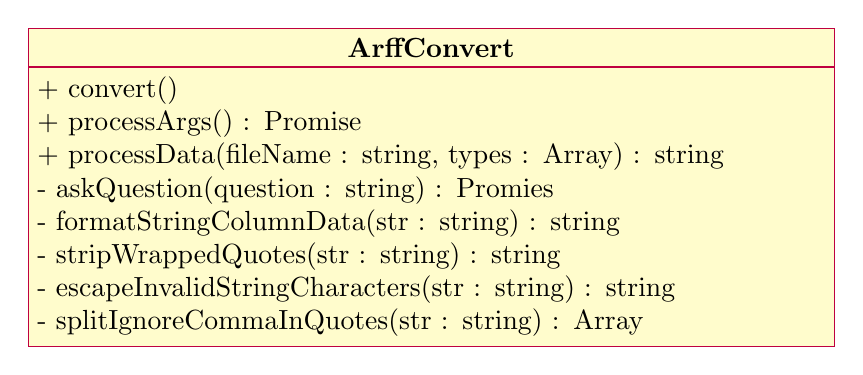
\begin{tikzpicture}
    \begin{class}[text width=10cm ]{ArffConvert}{0, 0}
      \operation{+ convert()}
      \operation{+ processArgs() : Promise}
      \operation{+ processData(fileName : string, types : Array) : string}
      \operation{- askQuestion(question : string) : Promies}
      \operation{- formatStringColumnData(str : string) : string}
      \operation{- stripWrappedQuotes(str : string) : string}
      \operation{- escapeInvalidStringCharacters(str : string) : string}
      \operation{- splitIgnoreCommaInQuotes(str : string) : Array}
    \end{class}
  \end{tikzpicture}
\end{center}

\subsubsection{convert()}
Convert is the function main call. It connects each function call together, reads the desired .csv file, and creates the new .arff file.

\subsubsection{processArgs()}
processArgs parses each command line argument passed in. It first extracts the fileName argument at index 0 from the argsArray, then it proceeds to loop throught each of the type arguments checking to see if they are date or enum types. If the type is date or enum the processArgs function asks the user what format or enum options to set that type to be. This function returns a promise to handle the asynchronous call that is used to get the users input.

\subsubsection{processData()}
The processData function call ensures that the data of the arff file is in the correct format. It loops throught every line of the .csv file wrapping strings in quotes, and replaces invalid characters. It then returns a string of the formatted file.

\subsubsection{Utility Functions}
There are five private utility functions. Four of them are used to format strings, and the fifth is a simple function to wrap the Node.js readline call.

\section{Experimental Data}


\end{document}
